\section{Methodology}
\label{sec:method}

The whole design comes down to one question: How should tasks be divided between the main agent and the background agents? Each is good at something the other can't do. The main agent knows the latest code, has learned the project's quirks and can talk to the user, but it built the code one request at a time and may be anchored on its early decisions. Background workers can try several structures in parallel, with nothing to protect, but they fall behind the conversation and can't ask the user questions. So the workers are given the full context up to that point, which lets them come in with a fresh perspective, and the judgment is left to the main agent and the user. That is why a design can be sent even when it is trailing behind the main conversation, since the main agent can reconcile it, and why a design only has to be worth reading, not ready to merge. The bar is still high: workers are prompted to come up with a better design, and several gates stop a bad or useless design from coming through. Ultimately, though, the main agent should think through what the background workers have given it and reach the final verdict with input and feedback from the user.

Figure~\ref{fig:flow} shows the four stages, and each section below explains what a stage does and how it got there.

\begin{figure}[t]
  \centering
  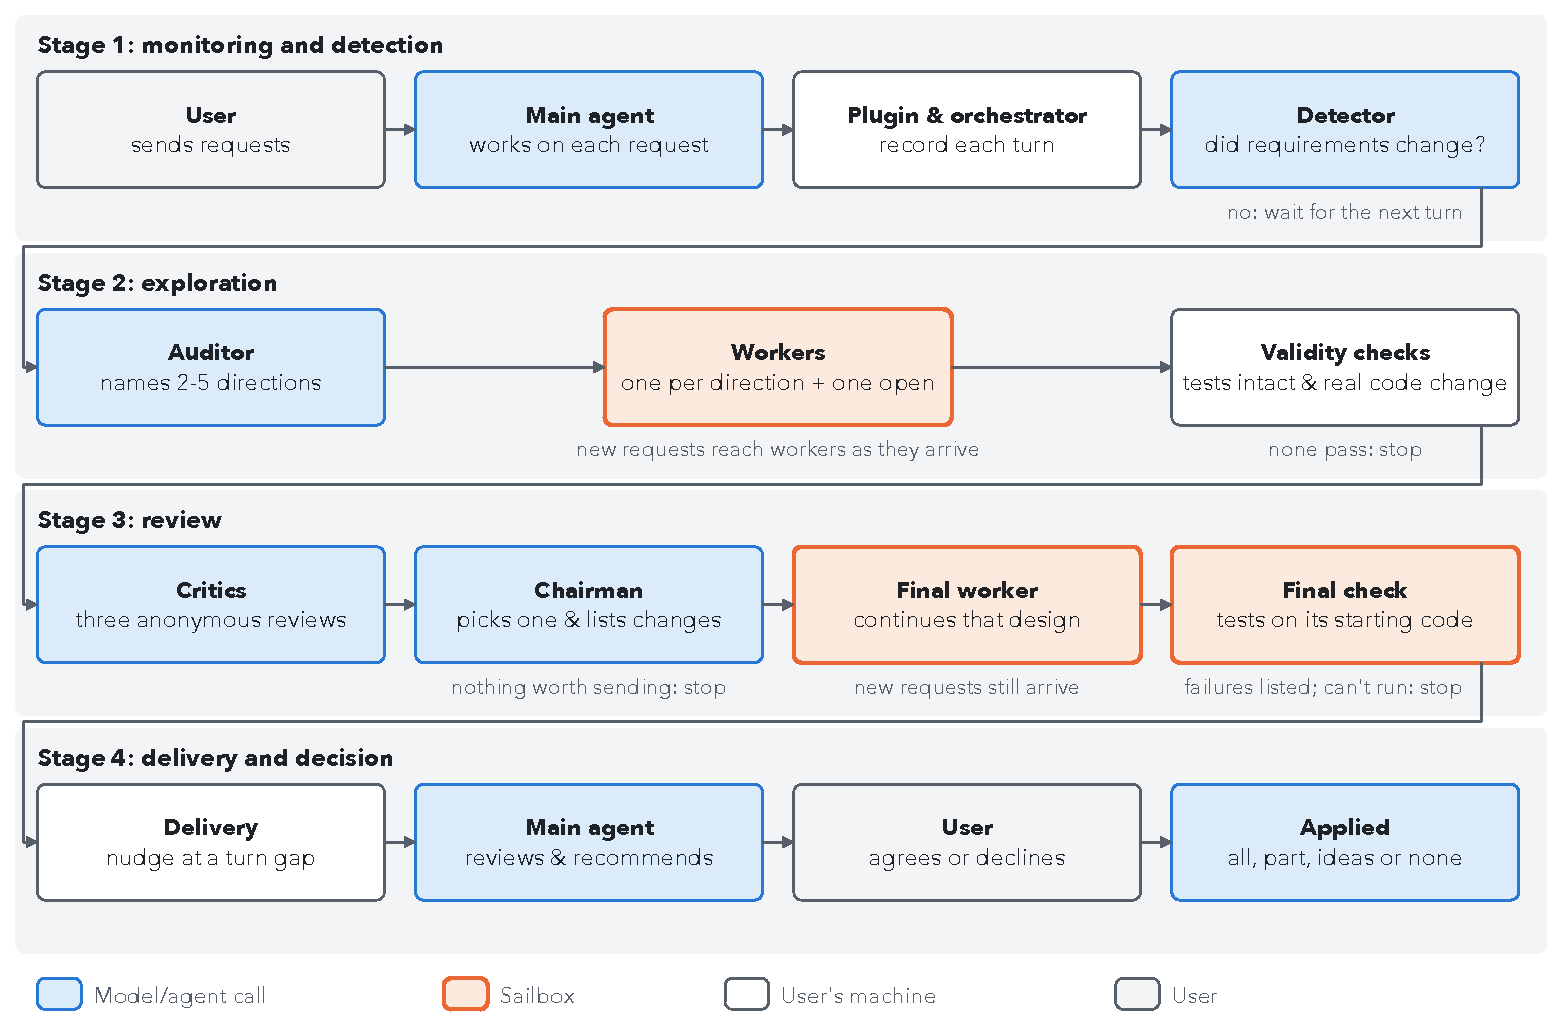
\includegraphics[width=0.8\linewidth]{fig_flow.pdf}
  \caption{The four stages of the system. Text under a box shows where a run can stop and where new requests reach a worker.}
  \label{fig:flow}
\end{figure}

\subsection{Stage 1: Monitoring and detection}

The user works with the main agent as usual. Hindsight uses OpenCode for this, watched through a plugin that forwards session events to the orchestrator, which runs on the user's machine. At the end of each turn, the orchestrator snapshots the folder to a private repository kept apart from the user's git history. The plugin never makes the session wait.

The harder problem is deciding when to act. One early design was an edge-case gate: models proposed edge cases the code might fail, ran them as real tests, and started the workers if any failed, which gave a trigger and a measurable target in one. The catch is that it's always possible to find an edge case. On a synthetic task designed to need no redesign, it delivered 17 nudges in 18 turns. It also pointed workers at problems a model had imagined instead of problems the user had, so it was dropped.

The opposite approach failed too. Another trigger asked the model whether it would build the code differently knowing everything, and it answered no on all 14 reviews across four benchmark tasks. Most of those requests added features without contradicting anything, and the code already worked. The current detector asks something narrower: does the latest request change or reverse something an earlier request specified, or something the code was built around (Figure~\ref{fig:request})? Purely additive requests count as no, and when unsure it answers yes. On a live run it said yes on 14 of 40 reviews, although a more robust evaluation would need a labeled set of ``redesign moments.''

\begin{figure}[t]
  \centering
  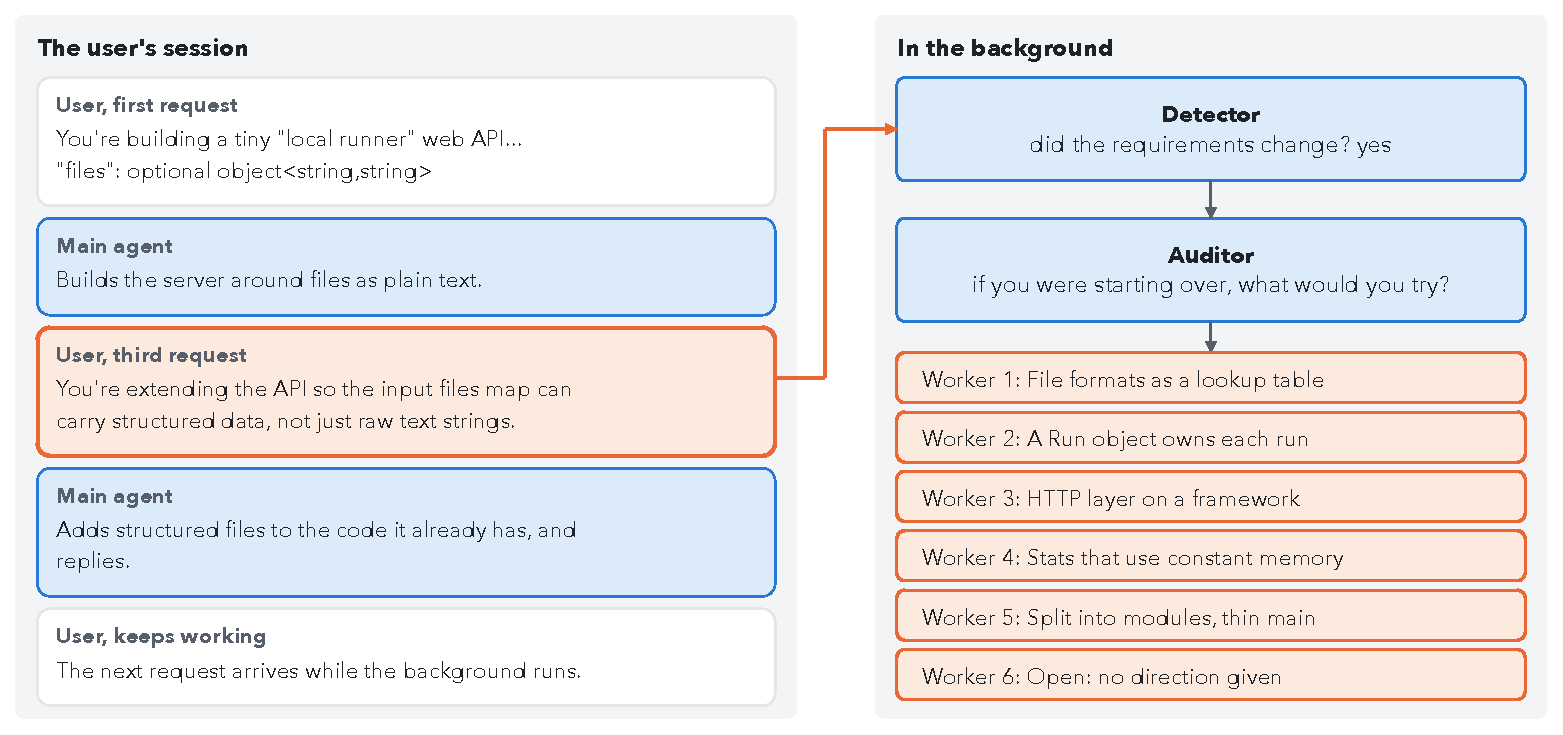
\includegraphics[width=0.9\linewidth]{fig_request.pdf}
  \caption{An illustrative example of a request that changes something the code was built around. The background starts while the session carries on. Messages are shortened from \code{execution_server}, a task from a public coding benchmark in which an agent builds a small web API for running code, and the directions are the ones the auditor named on that task.}
  \label{fig:request}
\end{figure}

\subsection{Stage 2: Exploration}

After a yes, an auditor names 2 to 5 directions a strong engineer would seriously consider if starting over. One worker builds each direction, and one more gets an open brief: nobody has picked a direction for it, so it is free to design whatever it would have built knowing everything. Each worker runs in its own Sailbox, a persistent Linux virtual machine billed for what it uses and free while asleep, with its own copy of the code. A worker can edit and run anything without going near the user's repository.

An earlier version used six fixed personas, such as a clean rewriter and a minimalist surgeon. They shared a step saying that leaving correct code alone was a useful result, and in one comparison 28 of 45 designs changed no real code. Now a worker has to restructure (``Handing back the same structure with a few fixes is not a result'') and has to say what its design makes better and what it costs. Letting the auditor set the number of workers means the team size follows the problem, though in practice it usually names close to the maximum.

Long-running workers raise the question of how to keep up with a conversation that doesn't stop. New user messages are delivered to every running worker, which reads them before finishing. Each session also runs only one background cycle at a time, since a second run would mostly repeat the first. The trade-off is that a weak run can stop a better one from starting.

Workers have a 45-minute time limit, which keeps runs feasible on complex tasks. This is a knob that can be tuned, and potentially set by the user, depending on cost and time constraints. A dropped connection continues the same conversation, and code present at the limit is kept and labeled unfinished. Two validity checks follow, using no model. One rejects weakened tests. The other requires a real change to product code, comparing Python by its syntax tree, because some designs only touched docstrings and config files.

\subsection{Stage 3: Review}

With several designs and no test that can say which structure is best, the review borrows the shape of Karpathy's llm-council~\cite{karpathy2025council}. Three critics, with the lenses requirements auditor, simplicity advocate and scope examiner, read the user's messages, the current code and each anonymized design. A chairman then picks one design to build on, or decides nothing is worth sending. It doesn't merge designs, because different structures rarely combine, but it lists what to change in the chosen design, which can include specific ideas borrowed from the others. A final worker starts with that design in place and makes those changes. Testing found that giving the final worker a design to build from, rather than asking it to redesign from a written plan, led to a better final design and better retained the workers' ideas.

The last step is a deliberately light check. Stricter checks would drop designs over changes that arrived late or over incompatibilities the main agent could resolve, and an early hard merge produced 48 false conflicts out of 48 proposals. So the check runs only against the code the design was built from, or runs the worker's own tests if the project has no suite, and a failure gets one retry. After that, the design goes out with its failures listed, because a test can fail only because it was tied to the old structure, and the main agent can tell the difference. Only a design that can't be run at all sends nothing.

\subsection{Stage 4: Delivery and decision}

At the next gap between turns, a nudge reaches the main agent, and the user gets a toast notification (Figure~\ref{fig:delivery}). The message is marked as coming from Hindsight and holds a one-sentence summary, an evidence line built by code, the background workers' own description labeled unverified, any messages the design missed, how far behind the design is, and the diff itself.

Delivery didn't start out this way. At first, a design needed a clean rebase and a test flip, then went straight to the user, all or nothing. Thinking through the relationship between the user, the main agent and the background system changed that. The main session doesn't wait, so suggestions will lag, which makes a strict, perfectly current patch the wrong thing to aim for, and the agent that has been in the code all along is the right reviewer.

The main agent reviews the design and recommends all of it, part of it, only its ideas, or none, and the user decides. The message asks the agent to change no code until the user agrees. Hindsight's own code only writes to the repository through an adoption tool, which takes a backup, runs tests and offers undo. Afterwards, the final worker's box goes to sleep, and the main agent can wake it to ask the background worker that built the design about it.

\begin{figure}[t]
  \centering
  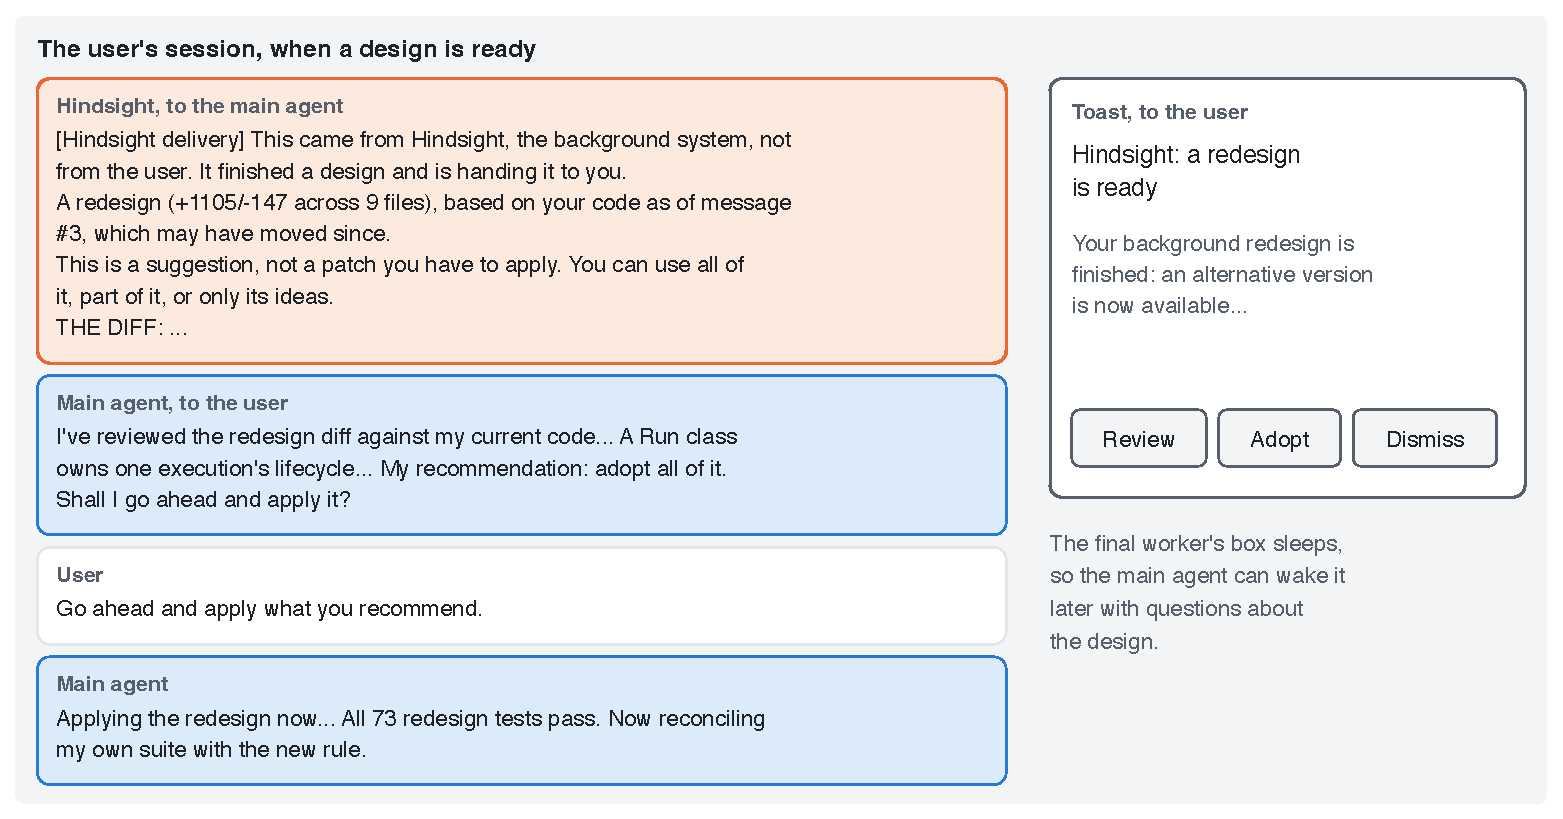
\includegraphics[width=0.9\linewidth]{fig_delivery.pdf}
  \caption{A design comes back. The main agent receives the diff and context, and the user gets a toast. Messages are shortened from \code{execution_server}, the web API task from Figure~\ref{fig:request}, where a simulated user gave the go-ahead. Benchmark runs have no desktop interface, so the toast is shown as designed.}
  \label{fig:delivery}
\end{figure}
